\chapter{Method}
\label{cha:Method}

 %- requirements, design, user study (if done)
 %- automating implementation?

This chapter goes through requirements definition and design stages. It is here, where one can find specification of the functional and non-functional requirements, use cases and a plan of general architecture of the system. 

\section{Requirements}

This section is devoted to stating requirements. Functional and non-functional requirements have been divided into two subsections. At the end a couple of constraints that the project has are mentioned.

\subsection{Functional requirements}
Functional requirements should define what the system ought to do. Below the main requirements are presented in the form of a list. 

The product shall:
\begin{itemize}
  \item properly recognize speech,
  \item create source code,
  \item modify source code,
  \item run a program,
  \item debug a program,
  \item allow navigation in the file,
  \item allow navigation in the workspace.
\end{itemize}

The system's main functionality can be stated as ``translating user's speech into an operation that is to be performed inside IDE''. Each particular requirement corresponds to one type of operation. In other words, the system should respond to user's input, which is always audio data. The resulting output is an action performed by the system. When the user wants, for example, to create a for loop, he/she has to speak out a proper sentence which the system should interpret. 

Because CodeSpeech is to allow writing programs by voice, of course it needs to be able to perform every task that is required in programming. It needs to provide a way to create source code, modify thereof, navigate inside files as well as in between files. Running and debugging the program are also inherent parts of programming, therefore should also be possible.

These requirements are a certain simplification, as \eg the term ``create source code'' could mean creation of variables, methods or other structures, similarly ``modify source code'' could mean deletion of a line, changing the name of the structure, adding a parameter \etc. Each of the requirements consists of many elements that could be stated on its own. For simplicity a generalization was made.

\subsection{Non-functional requirements}
Non-functional requirements describe what the system ought to be like. Below there is a list of the main characteristics that define a good implementation of the system.

The product shall:
\begin{itemize}
  \item be easy to use - to ensure high usability,
  \item interpret user’s natural English sentences - the system is directed towards English speakers,
  \item work with non-native speakers - there are many different accents and the system should work with most of them,
  \item be reliable - system should not crash or lose data,
  \item not perform many mistakes - to ensure usability and decrease frustration,
  \item have a way to correct mistakes - mistakes done either by the system or the user should have an easy way of being corrected,
  \item be intuitive - should require little time to be learned,
  \item inform about errors and a way to prevent them - user has to be always informed of what is happening,
  \item quickly respond to the user - to increase productivity,
  \item give precise feedback - user should be able to understand what has happened, might have an influence on speech recognition,
  \item must work with Eclipse IDE - system is intended to work as an Eclipse plugin,
  \item be easily available from within Eclipse Market - acquiring and installation of the system should be easy and almost automatic, 
  \item run on Windows OS,
  \item run on Linux OS.
\end{itemize}

\subsection{Constraints}
CodeSpeech has couple of constraints resulting from either its nature or technology used. The first obvious constraint is a need of a microphone. The program is heavily dependent on audio input cannot be used without a way to record voice. Another constraint related to that is a requirement of usage in a quiet environment. In order to increase performance of recognition ambient noise should be decreased to the minimum. One software constraint is Eclipse IDE with JDT (Java development Tools) installed on the workstation as the system is intended to be a plugin. Finally, because of the use of selected speech recognition tool, CodeSpeech requires an Internet connection.

\section{Use cases}

Below one can find enlisted use cases with short description. They depict different actions that can be performed from the user's point of view, such as the creation of the specific code structure, moving the cursor to a given line \etc In Fig. \ref{fig:useCases} a visualization in the form of UML Use Case diagram is presented. The main use cases are:

\begin{enumerate}
  \item Creating source code - most important part of programming. It involves: \eg
    \begin{itemize}
     \item creation of project elements, such as project, package, compilation unit,
     \item creation of programming structures, such as variables, methods definitions, invocations, loops, if conditions \etc
   \end{itemize}
  \item Modifying source code - due to mistakes or constant development process, modification of source code is inevitable. Examples of modification: 
    \begin{itemize}
     \item name, type changes,
     \item values assignment, initialization,
     \item addition, removal of method parameters/arguments,
     \item deletion of a structure.
   \end{itemize}
   
  \item Local navigation (in file) - placing a cursor in a specific position in a file:
  \begin{itemize}
     \item vertical navigation (between lines),
     \item optional: horizontal navigation (by character/nodes \eg parameter).
   \end{itemize}
   
  \item Global navigation (between files) - such as:
  \begin{itemize}
     \item selection of other projects in the workspace,
     \item opening another compilation unit for modifications.
   \end{itemize}
   
  \item Calling Eclipse commands - programming is not only writing source code, it also involves other actions, which nowadays are built-in into IDEs. That is why CodeSpeech was selected to be an extension of such an environment and provide a way to \eg:
    \begin{itemize}
     \item put/enable/disable a breakpoint into a specific line,
     \item compile program,
     \item run/debug program.
   \end{itemize}
\end{enumerate}

\begin{figure}[hbt!]
    \centering
    \fbox{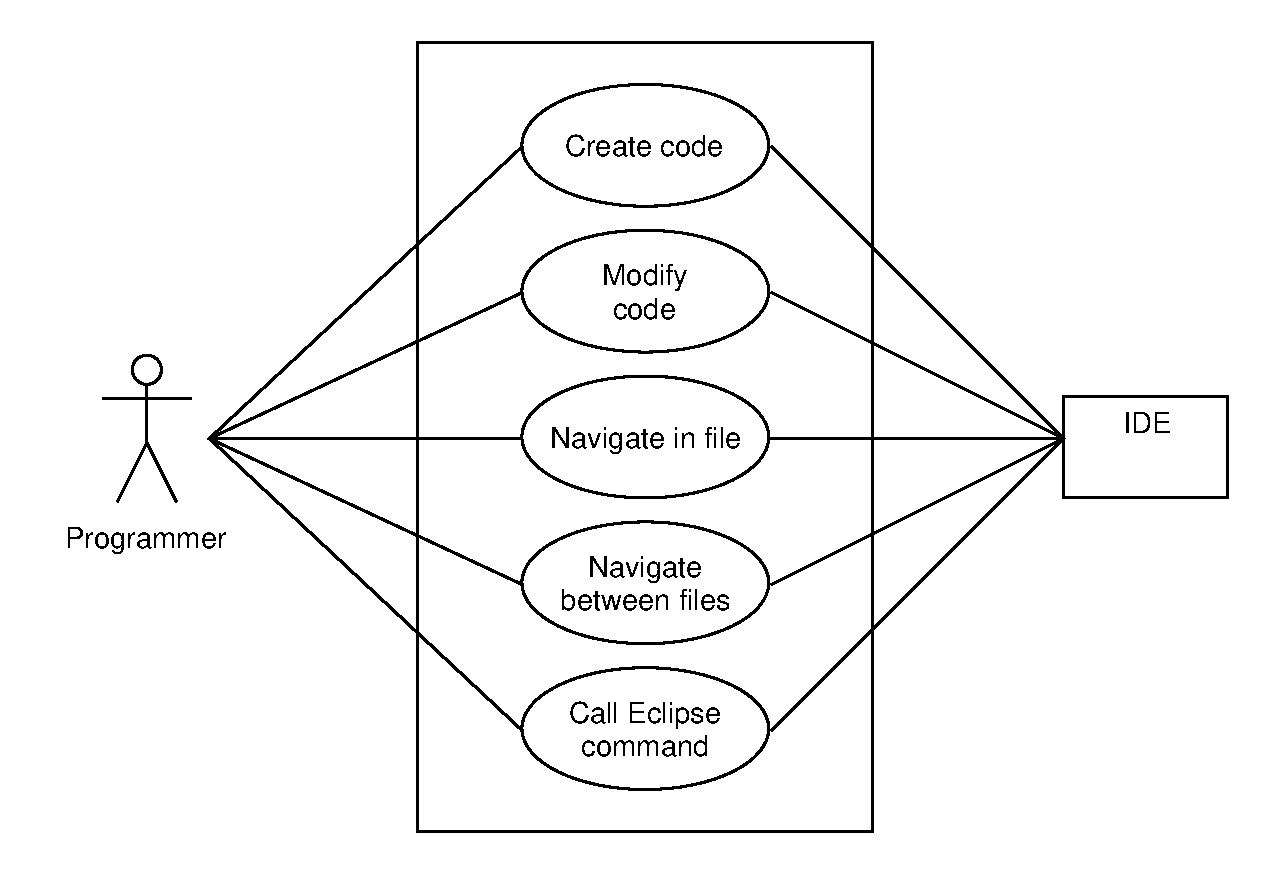
\includegraphics[width=\textwidth]{images/UseCaseDiagram.pdf}}
    \caption{Use Case diagram.}
    \label{fig:useCases}
\end{figure}
 
\leavevmode \\
\noindent
\textbf{Use Case 1}\\
User/actor name: Programmer\\
Description: Create code\\
Use Case Scenario:
\begin{enumerate}
  \item User speaks
  \item SR engine processes the audio signal and returns recognized speech in text 
  \item Plugin recognizes command
  \item Plugin performs operations on AST to create new code
  \item Plugin updates IDE
\end{enumerate}

\leavevmode \\
\noindent
\textbf{Use Case 2}\\
User/actor name: Programmer\\
Description:  Modify code \\
Use Case Scenario:
\begin{enumerate}
  \item User speaks
  \item SR engine processes the audio signal and returns recognized speech in text 
  \item Plugin recognizes command
  \item Plugin performs operations on AST to manipulate existing code
  \item Plugin updates IDE
\end{enumerate}

\leavevmode \\
\noindent
\textbf{Use Case 3}\\
User/actor name: Programmer\\
Description: Navigate in file\\
Use Case Scenario:
\begin{enumerate}
  \item User speaks
  \item SR engine processes the audio signal and returns recognized speech in text 
  \item Plugin recognizes command
  \item Plugin moves cursor to given position
\end{enumerate}

\leavevmode \\
\noindent
\textbf{Use Case 4}\\
User/actor name: Programmer\\
Description: Navigate between files\\
Use Case Scenario:
\begin{enumerate}
  \item User speaks
  \item SR engine processes the audio signal and returns recognized speech in text 
  \item Plugin recognizes command
  \item Plugin opens new editor and displays file's content
\end{enumerate}

\leavevmode \\ \\
\noindent
\textbf{Use Case 5}\\
User/actor name: Programmer\\
Description: Call IDE command\\
Use Case Scenario:
\begin{enumerate}
  \item User speaks
  \item SR engine processes the audio signal and returns recognized speech in text 
  \item Plugin recognizes command
  \item Plugin performs calls IDE's command
\end{enumerate}

\leavevmode

As it can be seen, the only thing required by the user to do is to speak the right command. The system then takes care of analyzing the speech and performing the right action.

\section{Design}
This section presents some ideas for the architecture of the system and its interface, discusses design choices backing them up with arguments, examples and summarises the advantages and disadvantages of these choices.

\subsection{System Architecture}
The structure of the system will consist of three main parts. One will be responsible for speech recognition, second for plugin management and the third for utterance interpretation. These are planned to be implemented in three structures: SpeechRecognizer, PluginManager and Interpreter, respectively. Fig. \ref{fig:architectureConcept} presents these components in simple UML diagrams.

\begin{figure}[hbt!]
\centering\small
\begin{tabular}{@{}c@{}} 
  \fbox{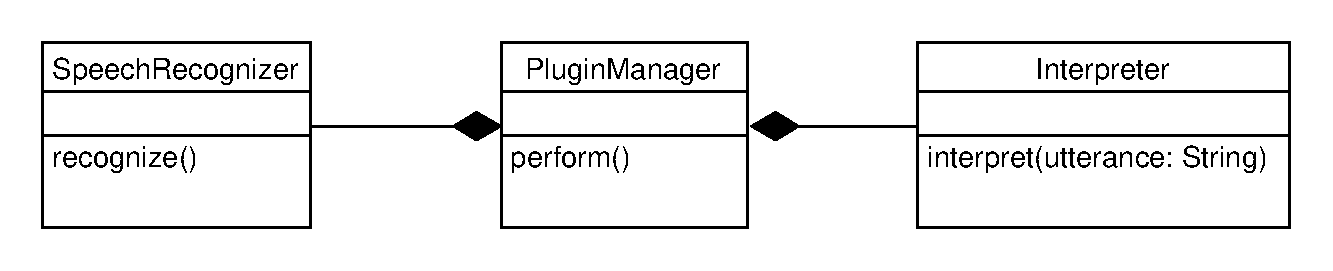
\includegraphics[width=\textwidth]{images/SimpleClassDiagram.pdf}} \\
  (a)  
  \\[10pt]
  \fbox{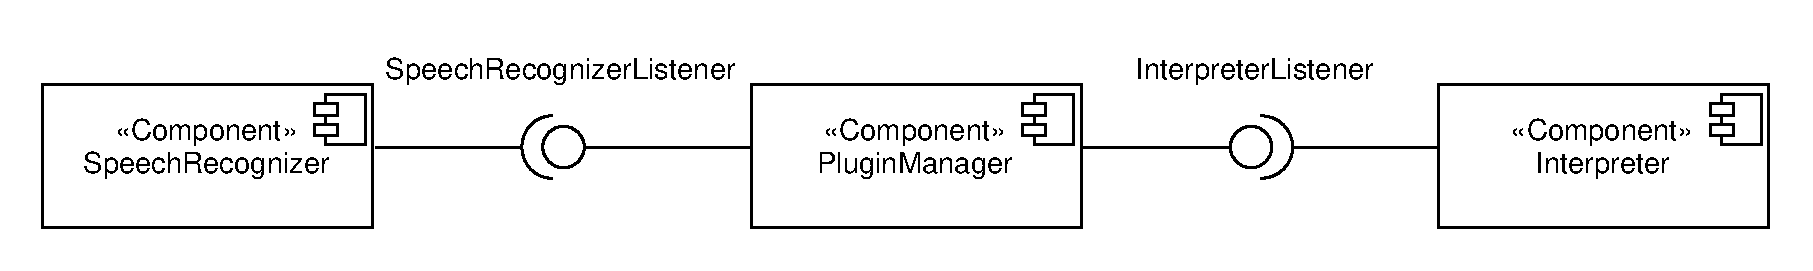
\includegraphics[width=\textwidth]{images/ComponentDiagram.pdf}} \\
  (b) 
  \end{tabular}
\caption{ Initial class diagram (a). Component diagram (b). }
\label{fig:architectureConcept}
\end{figure}

The main idea is like this: PluginManager is the main structure of the plugin so it initializes other structures and all necessary tools. This is due to the way Eclipse plugin structure look like. When plugin is on, SpeechRecognizer waits for audio input. When the user stops speaking, audio is treated by the implementation of currently used SR toolkit. When done, PluginManager is notified and receives the recognized utterance in the form of text. PluginManager then delegates the utterance to the Interpreter. Interpreter analyses the text and builds a proper Command object. Once the whole utterance has been walked through, the PluginManager is notified and receives the Command. Then, if everything is set, PluginManager executes the command and performs the action on IDE. The program can be interrupted and turned off at any stage of the recognition. Basic state diagram presenting the workflow is depicted in Fig. \ref{fig:stateDiagram}.

\begin{figure}[hbt!]
\centering\small
\begin{tabular}{@{}c@{}} 
  \fbox{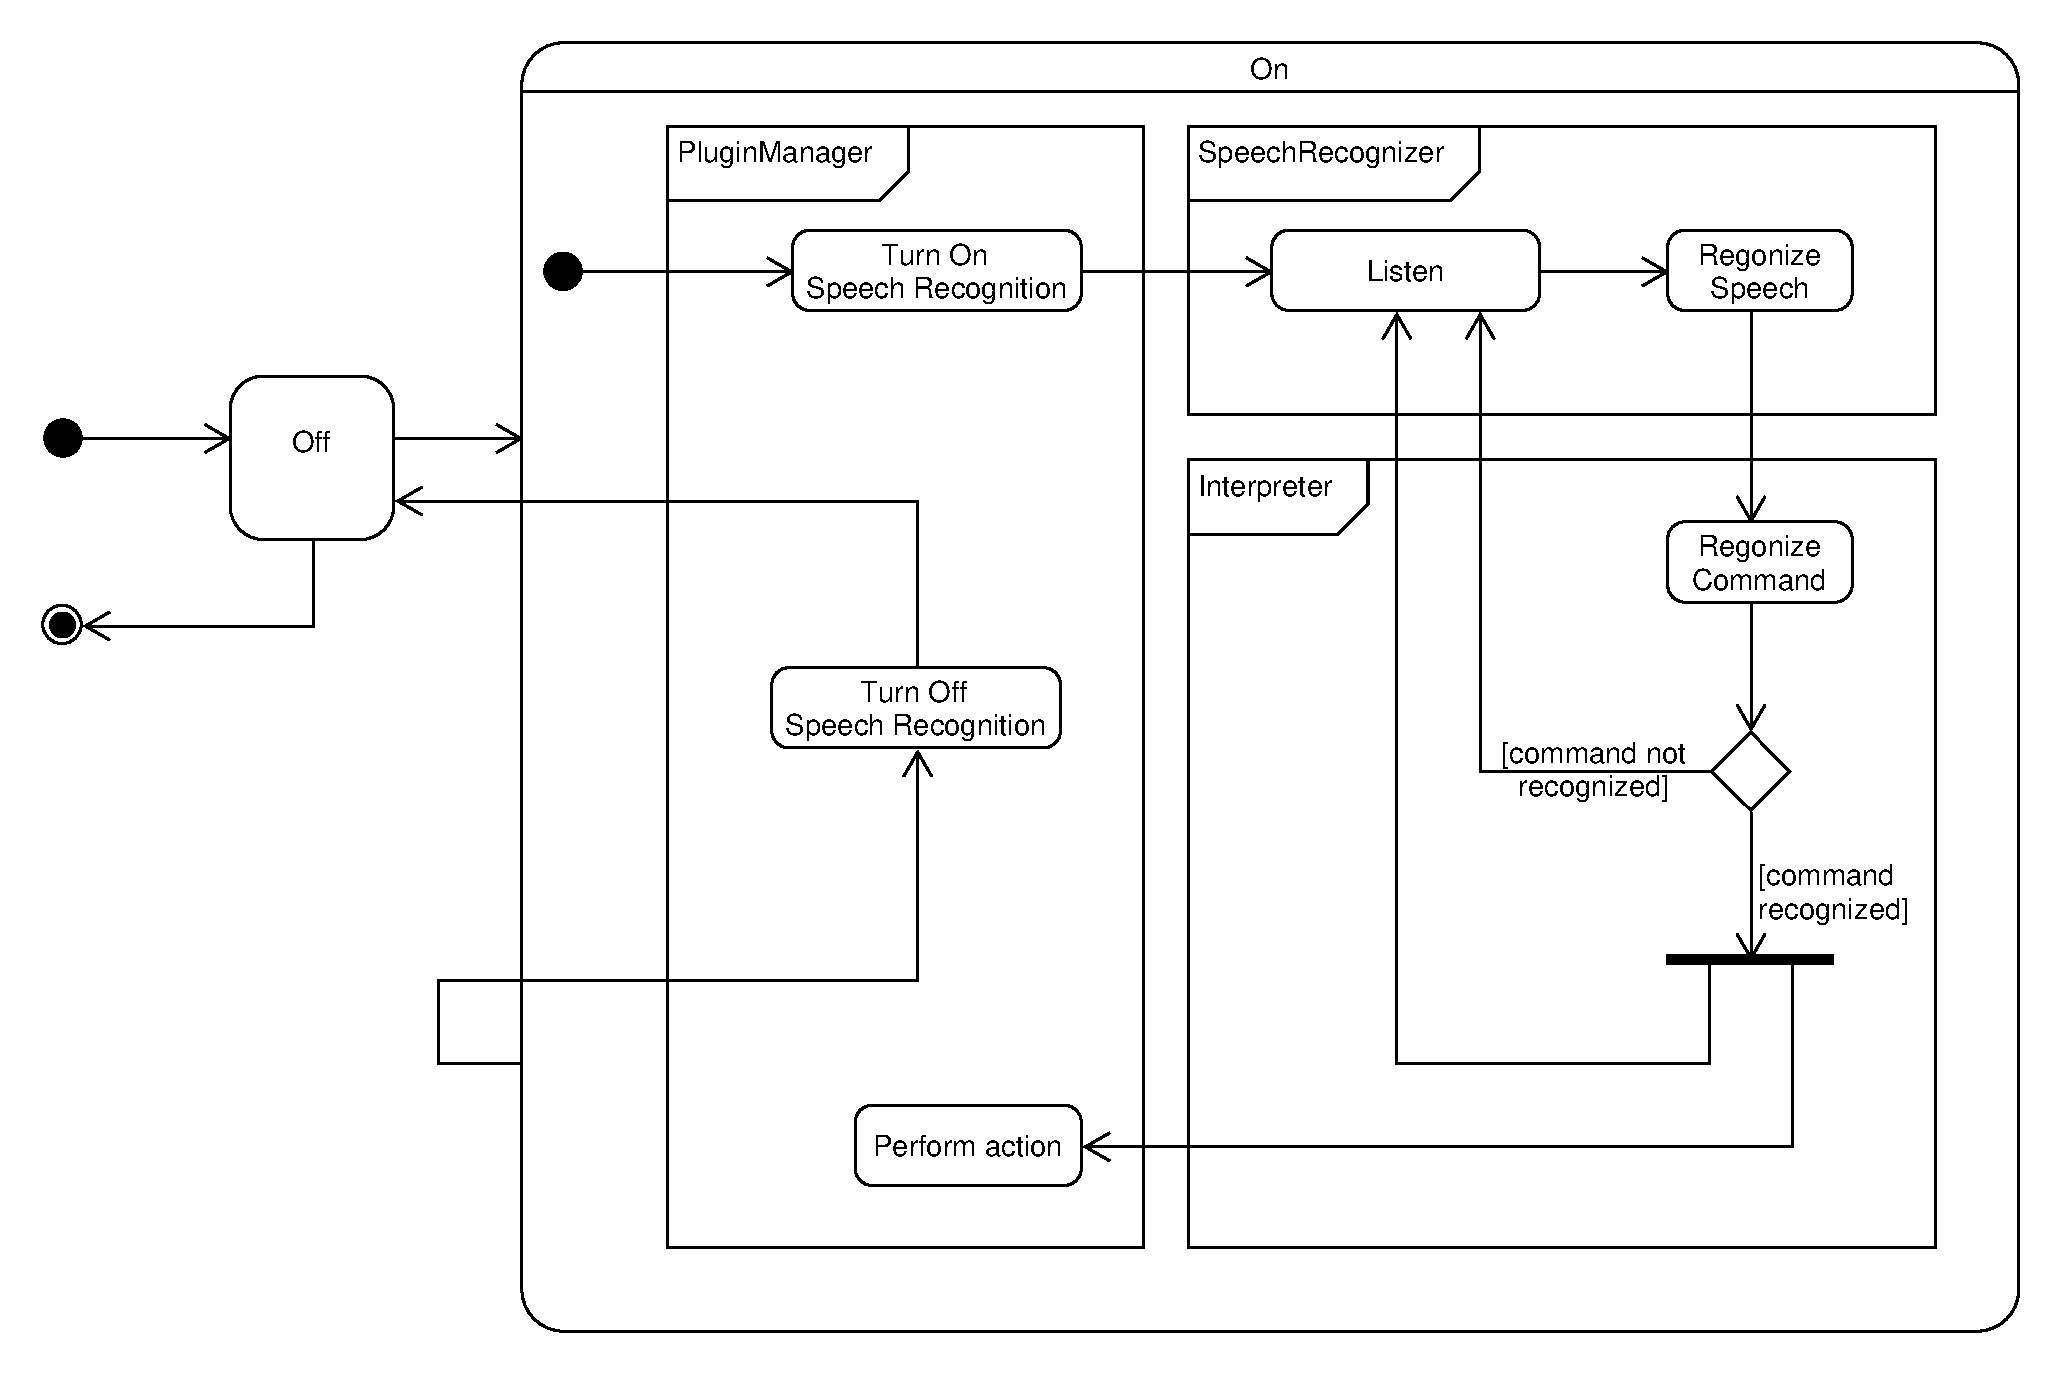
\includegraphics[width=\textwidth]{images/StateDiagram.pdf}}
  \end{tabular}
\caption{ State diagram of the program. }
\label{fig:stateDiagram}
\end{figure}

The system diagram is presented in Fig \ref{fig:systemDiagram}. Microphone does not have to be external, it can be one built into the laptop. Internet connection might be optional, depending on the system recognition tool that is being used. There might be a case in which a cloud service is utilized, and Internet connection is required. The system could be any which can run Eclipse IDE.

\begin{figure}[hbt!]
\centering\small
  \fbox{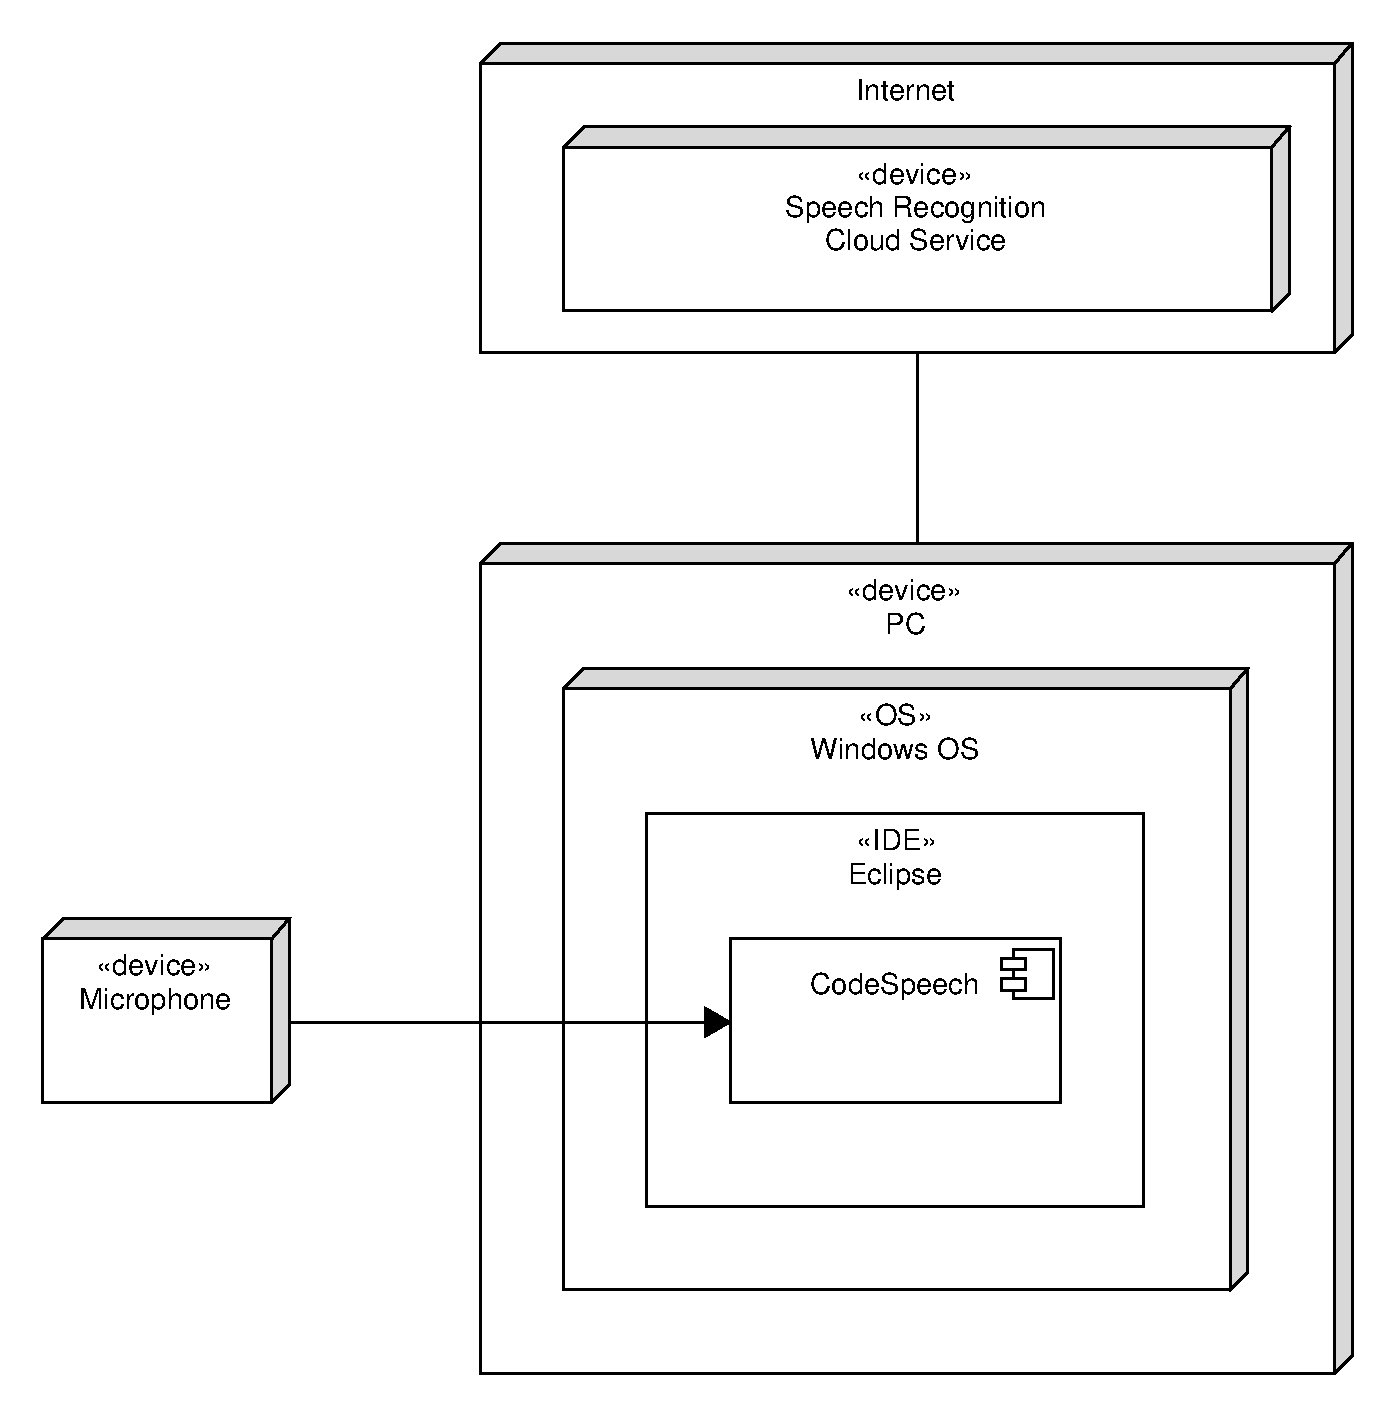
\includegraphics[width=\textwidth]{images/SystemDiagram.pdf}}
\caption{ System diagram.  }
\label{fig:systemDiagram}
\end{figure}

\subsection{Interface}

In order to have control over the plugin a button will be put into the toolbar menu. Clicking the button will toggle on and off programming by voice. Location of the button is presented in Fig. \ref{fig:toggleButton}. This method is a temporary solution because it still requires the use of mouse. In the future this way of interaction should be possibly replaced by activating via a specific command to decrease the need of using a mouse to zero. That will require to start up the programming by voice and activate microphone from the initialization of the IDE and wait for a specific voice command, such as \eg ``start voice programming''. Similarly ``stop voice programming'' would turn the main functionality off.  

\begin{figure}[hbt!]
    \centering
    \fbox{
\includegraphics[width=.6\textwidth]{images/ToggleButton.png}}
    \caption{Toggle button (in red frame) added to the menu to enable and disable programming by voice.}
    \label{fig:toggleButton}
\end{figure}

There exists an alternative way to control the plugin without the need of a mouse, namely a ``mouse grid'' tool that some of the available SR software, such as Windows SpeechRecognition, provide. Users can activate a grid that divides a screen into nine sections, and by speaking the number of a section where their interest lies, the grid scales and appears in that section as presented in Fig. \ref{fig:mouseGrid}. When one cell of a grid lies entirely in the position which they want to perform click on, it can be done simply speak a number of this cell and end with ``click'' word. That is a general idea behind this function, details might differ from one tool to another. After CodeSpeech is activated, external SR tool can be turned off. Stopping voice programming works analogically.


\begin{figure}[hbt!]
    \centering
    \fbox{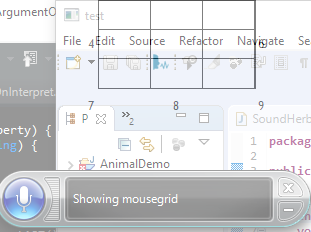
\includegraphics[width=.7\textwidth]{images/MouseGrid.png}}
    \caption{Mouse grid tool - alternative to the use of mouse build into Windows 10 SR.}
    \label{fig:mouseGrid}
\end{figure}

In addition a dialog box was introduced in the first iteration of the project in order to allow for introducing commands via text. This allows skipping the speech recognition phase and is to be used for debugging. This dialog is not planned to be used in the final version of the plugin. Fig. \ref{fig:debugDialog} depicts the command dialog box.

\begin{figure}[hbt!]
    \centering
    \fbox{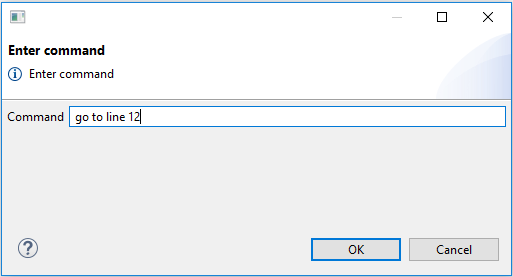
\includegraphics[width=.9\textwidth]{images/CommandDialogBox.PNG}}
    \caption{Command Dialog box that allows manual entry of commands.}
    \label{fig:debugDialog}
\end{figure}